%Johannes Grohmann
\newpage
\usecase{Besuchen der Startseite}
Der Nutzer öffnet zum ersten Mal die Startseite des Alumni-Portals und möchte sich grundsätzlich über das Portal und seine Funktionen informieren. Dadurch will er erfahren, ob eine Registrierung für ihn überhaupt Sinn ergibt. 

\usecasepart{Betrachten der Startseite}
Nach Eingeben der URL baut sich die Startseite auf (siehe Abbildung~\ref{fig:start}). Der Nutzer verschafft sich einen Überblick über die verfügbaren Funktionen und versucht einige von ihnen auszuprobieren. Er versucht zum Beispiel die Weltkarte anzuklicken oder wirft einen kurzer Blick auf die Stellenangebote. 

\begin{figure}[h]
	\centering
		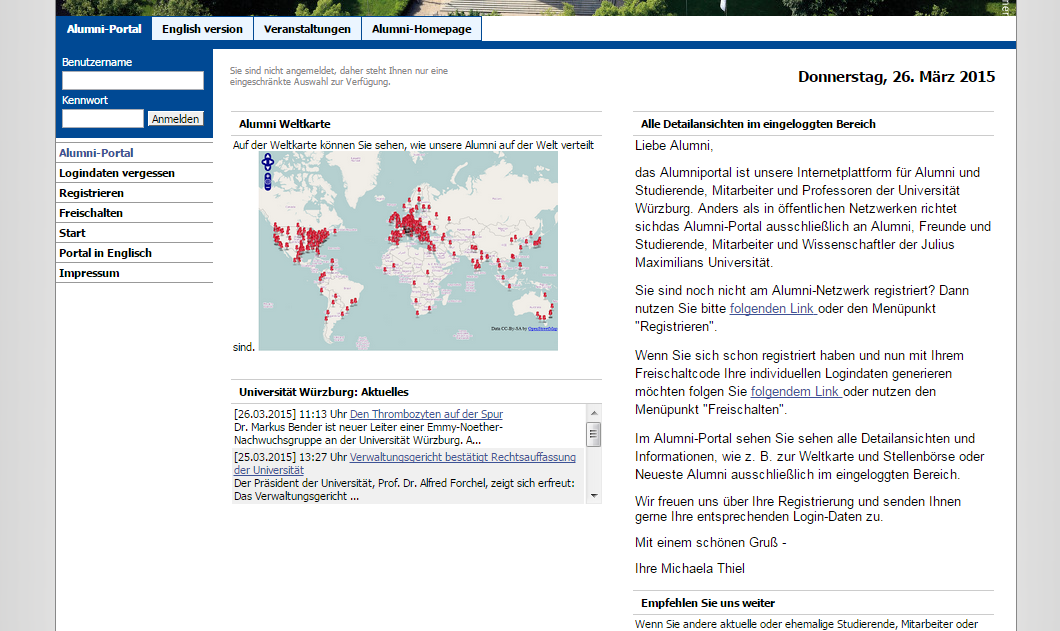
\includegraphics[width=\textwidth]{figures/startseite.png}
	\caption{Die Startseite des Alumni-Portals}
	\label{fig:start}
\end{figure}


\subsubsection*{Positive Beobachtungen}
Positiv zu bemerken ist, dass das Portal sich in puncto Farbgebung an das Corporate Design der Universität Würzburg anpasst. 
Auch das Titelbild, sowie die beiden Logos der Universität und des Alumni-Vereins sind passend eingebunden.
Weiterhin sind die Funktionalitäten sehr übersichtlich gehalten, um den Nutzer nicht von Beginn an mit Funktionen zu überfluten. 
Allgemein ist das Design sehr schlank und schlicht gehalten, um Nutzer nicht zu überfordern und abzuschrecken.

Der Rumpf der Seite ist schmal gehalten, um auch auf Geräten mit einer weniger hohen Auflösung korrekt angezeigt werden zu können. Der Rand ist dabei in neutralem Grau gehalten und wirkt angenehm passiv.

\problem{Unstrukturiertes Erscheinungsbild}
{Trotz des recht schlanken Designs wirkt die Webseite auf den ersten Blick recht unstrukturiert. Dies äußert sich in mehreren Punkten, die hier zusammengefasst werden. 
So werden insgesamt (exklusive Logos) 8 verschiedene Schrifttypen verwendet, die zudem nicht immer einen semantischen Unterschied signalisieren. In den beiden Textspalten finden sich beispielsweise zwei unterschiedliche Schrifttypen. 

Hinzu kommt ein viel zu kleiner Hinweistext in grau am Beginn der Seite, der darauf hinweist, dass nicht alle Funktionen ohne Login verfügbar sind.
In der linken Textspalte, ist zudem der Textsatz nicht überprüft worden, was dazu führt, dass das Wort \glqq sind\grqq~in die zweiten Zeile direkt neben die Weltkarte gesetzt wird, was auf den Nutzer sehr gequetscht wirkt.
Zusätzlich ist die Überschrift der rechten Spalte \emph{Alle Detailansichten im eingeloggten Bereich} unklar, unpassend und unverständlich und sorgt damit für Verwirrung.
}
{Durch das uneinheitliche Erscheinungsbild, wird es dem Nutzer erschwert sich auf der Seite zurecht zu finden. Dennoch sind nach längerem Suchen die Struktur und alle Funktionen der Seite erkennbar, das Problem ist also nicht besonders schwerwiegend, sondern nur geringfügig störend (Kategorie~1).
}
{Es wird eine Reduktion auf 3 bis 4 verschiedene Schrifttypen und weniger, aber dafür aussagekräftige Überschriften empfohlen. Zusätzlich mit einer deutlicheren Hervorhebung von Hinweistexten sollte dies das allgemeine Erscheinungsbild und den ersten Eindruck, den der Nutzer von der Startseite gewinnt, deutlich verbessern.
}\label{prob:start:erschbild}

\problem{Weltkarte ist nicht für Besucher verfügbar}
{Bei einem Blick auf die Startseite fällt sofort die ansprechende Weltkarte auf, siehe Abbildung \ref{fig:start}. 
Der Nutzer möchte die Karte anklicken und erwartet eine größere und interaktive Version der Weltkarte zur Verfügung zu haben.
Der Zugriff auf die Weltkarte wird einem Besucher jedoch (unverständlicherweise) nach dem Klick verwehrt und der Nutzer wird auf eine Login-Seite verlinkt. 
Dies stellt eine Dissonanz zwischen der Erwartung des Nutzers und dem Verhalten des Systems dar.
}{Da die Weltkarte derart auffällig platziert ist, lockt sie die Aufmerksamkeit des Nutzers an. Dieser wird durch die Nichtverfügbarkeit abgeschreckt. 
Die fehlende Funktionalität der interaktiven Weltkarte stellt deshalb einen schweren Fehler dar, da der Nutzer bereits hier wegen fehlender Motivation abbrechen könnte (Kategorie~4).}
{Die Weltkarte kann zweifellos auch ohne Login zugänglich und bedienbar gemacht werden.\footnote{Obwohl nicht Teil des eigentlichen Use-Cases, ist die Weltkarte außerdem auch Werbung und Aushängeschild der Universität Würzburg. Sie sollte auch für Nicht-Alumni und Interessenten der Universität verfügbar gemacht werden, da diese sich überhaupt nicht anmelden können.}
Dadurch fühlt sich der Nutzer nicht im \glqq Stöberverhalten\grqq ~beeinträchtigt.
}\label{prob:start:weltkarte}

\problem{Zweispaltiges Design}
{Der Text der Startseite ist in zwei Spalten aufgeteilt. Dies führt zu einer schlechteren Lesbarkeit, da zudem keine Hierarchie erkennbar ist, also beiden Spalten gleich viel Platz eingeräumt wird.
Dadurch wird kein Leitartikel erkennbar, was es für den Nutzer schwer macht in die Webseite einzusteigen. 
Durch die Seitenränder und das Seitenmenü findet eine weitere Einengung statt, sodass der Text stark in die Länge gezogen wird, der Nutzer somit weit nach unten scrollen muss.
Hinzu kommt, dass die linke Spalte deutlich weniger Text beinhaltet als die rechte Spalte, was dazu führt, das am Ende der Seite nur noch etwa ein Viertel der zur Verfügung stehenden Breite genutzt wird. Dies führt wiederum zu einer weiteren Streckung des Textes. 
}{Die Zweiteilung wirkt sehr ungeschickt und verhindert zudem, dass der gesamte Platz der Webseite genutzt werden kann. Es führt allerdings nicht zu einer Behinderung des Nutzers, weshalb es als leichtes Problem eingestuft werden kann (Kategorie~2).
}{Wichtig wäre hier vor allem eine klare Hierarchie vorzugeben, die sich auch in der Platzaufteilung zeigt. Dadurch wird die Aufmerksamkeit des Nutzers direkt auf diese Spalte gelenkt und es gibt einen klar erkennbaren Anfang der Seite.}\label{prob:start:design}

\problem{Scrollpanel in linker Spalte} 
{In der linken Spalte befindet sich ein Scrollpanel mit der Überschrift \emph{Aktuelles}. Dem Nutzer erscheint eben dieses jedoch vollkommen fehl am Platz.
Zunächst sind die Informationen im Contentbereich viel zu klein dargestellt und jede Nachricht ist auf 2 Zeilen begrenzt. Außerdem erübrigt sich der platzsparende Charakter eines Scrollpanels, da durch die rechte Spalte die Webseite ohnehin nach unten expandiert wird. 
Dies führt dazu, dass der Rest der linken Spalte leer bleibt, während der Nutzer im viel zu klein geratenen Panel nach unten scrollen muss.
}{
Der Sinn des gesamten Panels erschließt sich dem Nutzer keineswegs. Es spart keinen Platz, sondern führt nur dazu, dass der Nutzer gezwungen ist, selbst im Panel zu scrollen. Das führt zu Verärgerung und Verwirrung, da das Tool hier völlig falsch angewandt wurde (Kategorie~3).
}{
In diesem Fall, wäre es besser das Scrollpanel einfach wegzulassen und den Newsfeed \emph{Aktuelles} als Artikel unter der Weltkarte normal anzuzeigen. Gegebenenfalls kann das Scrollpanel auch so eingestellt werden, dass es sich bis zum Seitenende expandiert, also beide Spalten ausgeglichen lang sind. 
}\label{prob:start:panel}

\usecasepart{Betrachten der Menüs}
Im Folgenden untersucht der Nutzer die Startmenüs und ihre Funktionen etwas genauer. Zu diesem Zweck ist in Abbildung~\ref{fig:menu} das Menü noch einmal vergrößert dargestellt.

\begin{figure}[h]
	\centering
		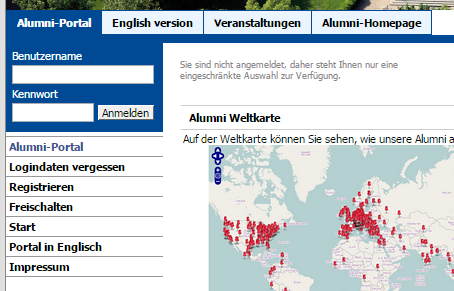
\includegraphics[width=\textwidth]{figures/menu.png}
	\caption{Eine vergrößerte Darstellung der Menüs der Startseite}
	\label{fig:menu}
\end{figure}


\subsubsection*{Positive Beobachtungen}
Die beiden Menüs sind in Umfang und Funktion recht übersichtlich gehalten, es wurde auf die Basisfunktionen reduziert. Dadurch sind alle wichtigen Menüpunkte schnell und einfach zu erreichen. 
Außerdem ist der derzeit aktive Menüpunkt immer deutlich markiert, so dass der Nutzer zu jedem Zeitpunkt weiß, auf welcher Seite er sich im Moment befindet.

\problem{Verwendung zweier Menüs}
{Zunächst fällt dem Nutzer auf, dass sowohl ein Header-Menü, als auch ein Menü am linken Seitenrand vorhanden sind. Das ist verwirrend, da auch keine semantische Trennung in den Funktionen beider Menüs vorhanden ist. 
}{Das Vorhandensein zweier Menüs an unterschiedlicher Stelle verwirrt den Nutzer. Da dennoch alle Funktionen verfügbar sind, ist das Problem nicht besonders schwerwiegend (Kategorie~2).
}{Hier wäre eine Reduktion auf ein Menü ratsam (vorzugsweise das Header-Menü). Dadurch sind alle verfügbaren Funktionen klar sortiert und somit zugänglicher. 
}\label{prob:start:menues}

\problem{Redundante Funktionen} 
{Die Menüpunkte \emph{Start} und \emph{Alumni-Hompage}, sowie \emph{Portal in Englisch} und \emph{English version} sind jeweils redundant in beiden Menüs mit unterschiedlicher Benennung angebracht, verfolgen aber den gleichen Zweck. Außerdem ist der Menüpunkt \emph{Alumni-Portal} in beiden Menüs vorhanden.
}
{Durch die doppelte Platzierung und unterschiedliche Benennung der Menüpunkte wird dem Nutzer ein semantischer Unterschied suggeriert, der nicht vorhanden ist. Das führt zwar zur Verwirrung, die Funktionen sind aber dennoch verfügbar und auffindbar (Kategorie~1).
}
{Die redundanten Menüpunkte können entfernt werden, um dem Nutzer eine klare Übersicht über die verfügbaren Funktionen zu geben. 
}\label{prob:start:funktionen}

\problem{Menüpunkt: Logindaten vergessen} 
{Die Funktion \emph{Logindaten vergessen} ist im Menü recht unüblich. Der Nutzer nimmt an, dass die Funktionen des Menüs zur Navigation dienen. Das Problem der vergessenen Logindaten passt nicht in diesen Kontext.
}
{Der Nutzer wird durch die zusätzliche/unnötige Funktion verwirrt und von seiner eigentlichen Intention abgelenkt (Kategorie~2).
}
{Die Funktion sollte in der Nähe der Login-Funktion angebracht werden, da sie nur in diesem Kontext gebraucht wird. Außerdem ist das mittlerweile auch die übliche Platzierung, an dem ein Nutzer sie zuerst suchen würde.
}\label{prob:start:pkt:login}

\problem{Menüpunkt: Registrieren}
{Der Menüpunkt \emph{Registrieren} ist nicht im üblichen Kontext in der Nähe des Anmeldefensters angeordnet. Bei einem Klick öffnet sich ein Untermenü, das dem Nutzer zwei Optionen bietet: \emph{Registrieren} und \emph{Freischalten}.
Die Funktion \emph{Freischalten} ist vollkommen unklar. Der Nutzer weiß nicht, was die Funktion bewirkt oder wofür sie da ist. Auch der Unterschied zwischen Registrieren und Freischalten wird nicht deutlich.
}{Die Funktion ist nicht in ihrem üblichen Kontext angeordnet. Der Nutzer wird zudem durch die zusätzliche/unnötige Funktion verwirrt. Es entsteht der Eindruck, zur erfolgreichen Registrierung eine weitere Aktion ausführen zu müssen (Kategorie~3).}
{Die Registrierungsfunktion sollte in den Kontext des Anmeldefensters verschoben werden. Außerdem muss die Funktion des Freischaltens deutlicher erklärt werden. Alternativ wäre ein Zugang zum Freischalten auch nur mittels einem in der Registrierungsmail verschickten Hyperlink oder eine direkte Verlinkung nach dem ersten erfolgreichen Login denkbar.
}\label{prob:start:pkt:reg}

\problem{Menüpunkt: Freischalten} 
{Die Funktion Freischalten ist erstens bereits im Menü vorhanden, zweitens ist die Funktion dem Nutzer hier nicht klar (siehe Abschnitt~\ref{prob:start:pkt:reg}). 
Zusätzlich verlinken die beiden Funktionen mit dem Titel \emph{Freischalten} auf verschiedene Seiten, die aber beide die gleiche Funktion erfüllen. Für den Nutzer ist das allerdings nicht ersichtlich, da es sich um zwei verschiedene Links handelt.
}
{Durch den Mangel an Information und des Vorhandenseins zweier verschiedener Links, wird dem Nutzer zudem suggeriert es handele sich bei \emph{Freischalten} um zwei verschiedene Funktionen (Kategorie~3).
}
{
Da die Funktion bereits einmal im Menü vorhanden ist, genügt hier die Reduktion auf eine der beiden Optionen.
}\label{prob:start:pkt:frei}

\problem{Menüpunkt: Start} 
{Im linken Seitenmenü taucht zusätzlich ein weiterer Menüpunkt \emph{Start} auf. Auch hier ist die Funktion überhaupt nicht klar. Der Nutzer würde erwarten auf die Startseite der Webseite verlinkt zu werden, es geschieht jedoch eine Weiterleitung auf die Alumni-Hompage. 
}
{Dem Nutzer ist sich überhaupt nicht über die Funktion und deren Effekt im Klaren, was zu Verwirrung führt (Kategorie~3).
}
{Da der Menüpunkt ohnehin redundant mit der Funktion \emph{Alumni-Homepage} im Header-Menü ist, kann er ohne weiteres entfernt werden.
}\label{prob:start:pkt:start}

\problem{Menüpunkt: Portal in Englisch} 
{Der Menüpunkt \emph{Portal in Englisch} wirkt fehl am Platz. Sollte der Nutzer tatsächlich nach einer Übersetzung der Seite suchen, würde er dies rechts oben in der Ecke oder an sonstigen exponierten oder markanten Stellen tun. 
Der Nutzer stolpert hier im Menü nur über den Punkt, weil er ihn nicht an dieser Stelle erwartet hätte.
}
{Da der Menüpunkt recht unmissverständlich ist, hält er den Nutzer nicht lange auf (Kategorie~1).
}
{Die Funktion sollte in die rechte obere Ecke, neben anderen Sprachoptionen eingegliedert werden, wo der Nutzer sie erwarten würde.
}\label{prob:start:pkt:eng}

\problem{Menüpunkt: Impressum} 
{Die Funktion \emph{Impressum} im linken Seitenmenü wirkt ebenfalls fehl am Platz. Der Nutzer erwartet ein Impressum am Fuß der Seite, eine eigene Funktion im Menü lässt dieses schnell überladen wirken.
}
{Das Menü wird um eine unnötige Funktion erweitert, die schnell zum Überladen der Funktionen führen kann, der Nutzer findet das Impressum allerdings trotzdem falls er danach sucht (Kategorie~1).
}
{Das Impressum sollte nicht als Menüpunkt, sondern an den Fuß der Seite eingebunden werden. Dies hat sich als de-facto Standard etabliert, sodass der Nutzer es schneller findet, wenn er danach sucht.
Außerdem wird das Impressum so auch auf jeder Seite angezeigt und nicht nur auf der Startseite verlinkt. 
}\label{prob:start:pkt:imp}

\problem{Pop-Up Fenster} 
{Mehrere Aktionen der Menüs sind als Pop-Up Funktionen implementiert. Durch Klick auf \emph{Start}, \emph{Portal in Englisch}, \emph{English version} und \emph{Alumni Portal} öffnet sich ein Pop-Up Fenster, das von modernen Browsern grundsätzlich blockiert wird. 
Der Nutzer bekommt dies meistens nicht einmal mehr mit. Stattdessen erscheint nur ein kleiner Text auf der Seite, der darauf hinweist, dass die Seite in einem externen Fenster geöffnet wurde mit einem Link, um das öffnen manuell auszuführen.
Das Ergebnis ist, dass der Nutzer zweimal klicken muss, um auf die gewünschte Seite zu kommen.
}
{Da Pop-Ups in der Regel geblockt werden, ist das also eine klare Dissonanz zwischen den Erwartungen des Nutzers (Ein neues Fenster öffnet sich) und der Reaktion des Systems (Es wird nur ein kleiner Hinweistext angezeigt). Da Pop-Ups auf modernen Seiten im Grundsatz vermieden werden, stellt dies einen groben Fehler dar, da es Nutzer dazu bringen kann, aufgrund von fehlendem Feedback abzubrechen (Kategorie~4).
}
{Hier sollte auf die Verwendung von Pop-Ups grundsätzlich verzichtet werden.
}\label{prob:start:popup}

\problem{Dynamisches Seitenmenü} 
{Das Seitenmenü ist dynamisch an das Header-Menü gekoppelt. Das bedeutet, wenn der Nutzer durch das Header-Menü auf eine andere Seite wechselt, ändern sich die angebotenen Funktionen im Seitenmenü. Das ist äußerst problematisch, da für den Nutzer ohne ersichtlichen Grund wichtige Funktionen, wie \emph{Registrieren} plötzlich nicht mehr zur Verfügung stehen. Es ist auch nicht ersichtlich, wie es möglich ist, diese Funktionen wieder zu aktivieren.
Zusätzlich ist das Seitenmenü auf allen Seiten außer der Startseite völlig funktionslos. 
}
{Das plötzliche Verschwinden wichtiger Funktionen, kann dazu führen, dass der Nutzer den Use-Case nicht beenden kann und abbricht (Kategorie~4).
}
{Das Seitenmenü sollte statisch bleiben und auf jeder der Unterseiten die gleichen Funktionen anbieten.
}\label{prob:start:seitenmenue}

\subsubsection*{Fazit: Seitenmenü}
Das linke Seitenmenü hat sich als fehlerhaft und überflüssig gezeigt. 
Die redundanten Funktionen \emph{Alumni-Portal}, \emph{Portal in Englisch} und \emph{Start} sollten nur noch im Header-Menü angezeigt werden. Die Funktionen \emph{Logindaten vergessen}, \emph{Registrieren} und \emph{Freischalten} wären besser im Anmeldefenster untergebracht und das Impressum sollte an den Fuß der Seite.
Somit wäre jede Funktion des Seitenmenüs ausgelagert und das Menü kann entfernt werden, wie bereits in Abschnitt \ref{prob:start:menues} vorgeschlagen.
